\documentclass{standalone}
\usepackage{tikz}
\usepackage{tikzscale}
\usetikzlibrary{arrows}
\usetikzlibrary{arrows.meta}
\usetikzlibrary{patterns}
\usetikzlibrary{shapes}
\usetikzlibrary{calc}
\usetikzlibrary{matrix}
\usetikzlibrary{positioning}
\usepackage{calc}
\usetikzlibrary{calc,trees,positioning,arrows,fit,shapes}

\usepackage{tkz-euclide}
\usetikzlibrary{
	angles,
	quotes,
}
\usepackage{pgfplots}

\begin{document}

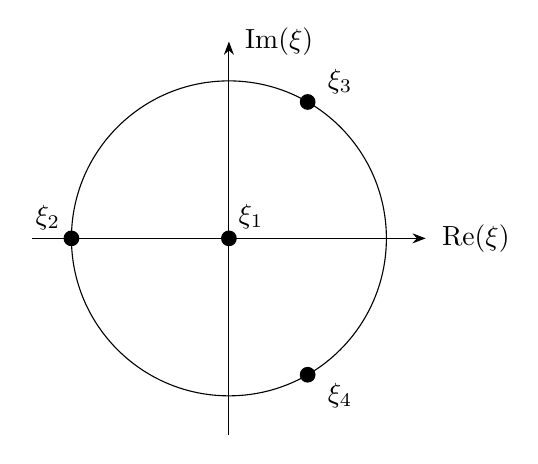
\begin{tikzpicture}
    [   baseline={([yshift=-1ex]current bounding box.north)}
    ,   > = Stealth
    ]
    \draw[->] (-25mm,0mm) -- (25mm,0mm);
    \draw[->] (0mm,-25mm) -- (0mm,25mm);
    \node[inner sep = 0pt, anchor = west] at (27mm,0mm) {Re$(\xi)$};
    \node[inner sep = 0pt, anchor = west] at (2mm,25mm) {Im$(\xi)$};
    \draw (0mm,0mm) circle (20mm);

    \coordinate (xi1) at (0:0mm);
    \fill (xi1) circle (1mm);
    \node[anchor = south west] at (xi1) {$\xi_1$};

    \foreach\x/\a/\d in {2/180/south,3/60/west,4/300/west}
    {
        \fill (\a:20mm) circle (1mm);
        \node[anchor = \d, inner sep = 1mm] at (\a:23mm) {$\xi_\x$};
    }
\end{tikzpicture}


\end{document}
